% CREATED BY DAVID FRISK, 2016
\chapter{Results}
Due to computational constraints, we constrain ourselves to 7 Atari games.
All chosen games are solvable by DQN or Rainbow, but vary in visual complexity
and control problem difficulty.
In particular, the selected games are: 
\begin{enumerate}
		\item Breakout
		\item Enduro
		\item Ms Pacman
		\item Pong
		\item Qbert
		\item Seaquest
		\item Space Invaders
\end{enumerate}

Because we can only indirectly gauge the effect of various metrics through 
final algorithm performance, the primary metric of interest is obtained 
return in relation to the number of training iterations.
Due to different reward scaling, we keep results on different games in separate graphs.
We further divide the results into those pertaining to different hypotheses
in order to avoid line clutter.
As a final note, the results for each particular setting are \textbf{single-runs}.
Generally speaking, this is not adequate due to high pseudorandom number generator seed 
dependence. Depending on the problem, 3-10 runs are averaged, or the best one is selected,
in order to tackle the problem.

\section{Effectiveness of pretrained encoders}
To begin, we first need to estimate the possible sample-efficiency gains.
This is done by comparing returns per training step between only reinforcement learning
and only reinforcement learning where training starts with a encoder
trained from the first reinforcement learning-only run.
Because we chose games which can be essentially solved with only reinforcement learning,
the encoder of a network trained with reinforcement learning should serve
as an ideal pretrained encoder.
\begin{figure}[!t]
  \captionsetup[subfloat]{position=top,labelformat=empty}
  \centering
  \subfloat[]{  \resizebox{0.4\textwidth}{!}{% This file was created by matlab2tikz.
%
%The latest updates can be retrieved from
%  http://www.mathworks.com/matlabcentral/fileexchange/22022-matlab2tikz-matlab2tikz
%where you can also make suggestions and rate matlab2tikz.
%
\definecolor{blue}{RGB}{76,100,135}
\definecolor{red}{RGB}{153,0,0}
\definecolor{yellow}{RGB}{227,178,60}
\definecolor{mycolor1}{rgb}{0.00000,0.44700,0.74100}%
\definecolor{mycolor2}{rgb}{0.85000,0.32500,0.09800}%
\definecolor{mycolor3}{rgb}{0.92900,0.69400,0.12500}%
%
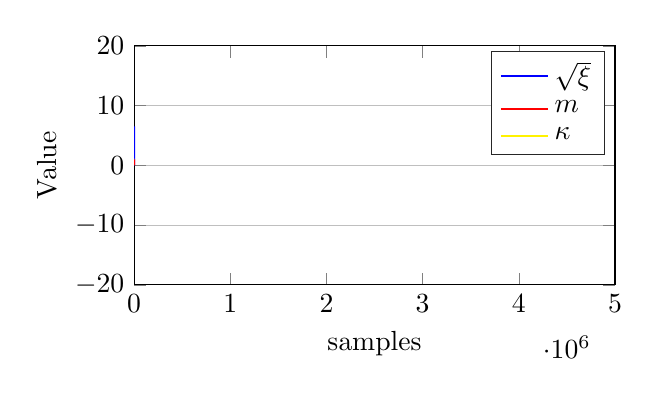
\begin{tikzpicture}

\begin{axis}[%
% width=4.634in,
width=6.634in,
height=3.612in,
at={(2.596in,2.358in)},
% scale only axis,
xmin=0,
xmax=5000000,
xlabel style={font=\color{white!15!black}},
xlabel={samples},
xlabel near ticks,
ymin=-20,
ymax=20,
ylabel style={font=\color{white!15!black}},
ylabel={Value},
ylabel near ticks,
ymajorgrids,
scale=0.4,
axis background/.style={fill=white},
legend style={legend cell align=left, align=left, draw=white!15!black}
]
\addplot [color=blue, line width = 0.25mm]
  table[row sep=crcr]{%
1	0\\
0.99	0.0142133212704263\\
0.98	0.0285709426850902\\
0.02	5.53243599059204\\
0.01	6.51269413406059\\
};
\addlegendentry{$\sqrt{\xi}$}

\addplot [color=red, line width = 0.25mm]
  table[row sep=crcr]{%
1	1\\
0.99	0.99\\
0.98	0.98\\
0.02	0.02\\
0.01	0.01\\
};
\addlegendentry{$m$}

\addplot [color=yellow, line width = 0.25mm]
  table[row sep=crcr]{%
1	1\\
0.99	1\\
0.98	1\\
0.97	1\\
0.96	1\\
0.03	1\\
0.02	1\\
0.01	1\\
};
\addlegendentry{$\kappa$}

\end{axis}
\end{tikzpicture}%
}} 
  \subfloat[]{  \resizebox{0.4\textwidth}{!}{% This file was created by matlab2tikz.
%
%The latest updates can be retrieved from
%  http://www.mathworks.com/matlabcentral/fileexchange/22022-matlab2tikz-matlab2tikz
%where you can also make suggestions and rate matlab2tikz.
%
\definecolor{blue}{RGB}{76,100,135}
\definecolor{red}{RGB}{153,0,0}
\definecolor{yellow}{RGB}{227,178,60}
\definecolor{mycolor1}{rgb}{0.00000,0.44700,0.74100}%
\definecolor{mycolor2}{rgb}{0.85000,0.32500,0.09800}%
\definecolor{mycolor3}{rgb}{0.92900,0.69400,0.12500}%
%
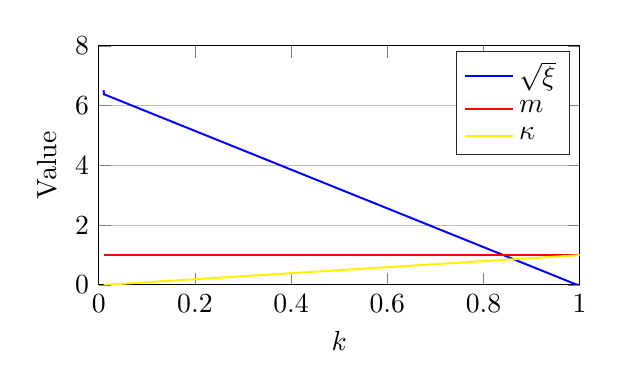
\begin{tikzpicture}

\begin{axis}[%
% width=4.634in,
width=6.634in,
height=3.612in,
at={(2.596in,2.358in)},
% scale only axis,
xmin=0,
xmax=1,
xlabel style={font=\color{white!15!black}},
xlabel={$k$},
xlabel near ticks,
ymin=0,
ymax=8,
ylabel style={font=\color{white!15!black}},
ylabel={Value},
ylabel near ticks,
ymajorgrids,
% scale=0.5,
scale=0.4,
axis background/.style={fill=white},
legend style={legend cell align=left, align=left, draw=white!15!black}
]
\addplot [color=blue, line width = 0.25mm]
  table[row sep=crcr]{%
1	0\\
0.999009009009009	0.00140216778227743\\
0.998018018018018	0.00280572716902405\\
0.997027027027027	0.00421068092522594\\
0.996036036036036	0.00561703182411782\\
0.995045045045045	0.00702478264721581\\
0.994054054054054	0.00843393618435142\\
0.010990990990991	6.37906390177465\\
0.01	6.51269413406059\\
};
\addlegendentry{$\sqrt{\xi}$}

\addplot [color=red, line width = 0.25mm]
  table[row sep=crcr]{%
1	1\\
0.999009009009009	1\\
0.998018018018018	1\\
0.997027027027027	1\\
0.01	1\\
};
\addlegendentry{$m$}

\addplot [color=yellow, line width = 0.25mm]
  table[row sep=crcr]{%
1	1\\
0.999009009009009	0.998019000081162\\
0.998018018018018	0.996039964288613\\
0.997027027027027	0.994062892622352\\
0.010990990990991	0.000120801882964045\\
0.01	0.0001\\
};
\addlegendentry{$\kappa$}

\end{axis}
\end{tikzpicture}%
}}\\
  \vspace{-1cm}
  \subfloat[]{  \resizebox{0.4\textwidth}{!}{% This file was created by matlab2tikz.
%
%The latest updates can be retrieved from
%  http://www.mathworks.com/matlabcentral/fileexchange/22022-matlab2tikz-matlab2tikz
%where you can also make suggestions and rate matlab2tikz.
%
\definecolor{blue}{RGB}{76,100,135}
\definecolor{red}{RGB}{153,0,0}
\definecolor{yellow}{RGB}{227,178,60}
\definecolor{mycolor1}{rgb}{0.00000,0.44700,0.74100}%
\definecolor{mycolor2}{rgb}{0.85000,0.32500,0.09800}%
\definecolor{mycolor3}{rgb}{0.92900,0.69400,0.12500}%
%
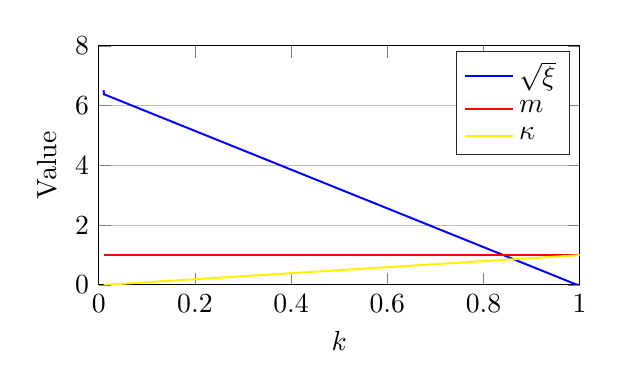
\begin{tikzpicture}

\begin{axis}[%
% width=4.634in,
width=6.634in,
height=3.612in,
at={(2.596in,2.358in)},
% scale only axis,
xmin=0,
xmax=1,
xlabel style={font=\color{white!15!black}},
xlabel={$k$},
xlabel near ticks,
ymin=0,
ymax=8,
ylabel style={font=\color{white!15!black}},
ylabel={Value},
ylabel near ticks,
ymajorgrids,
% scale=0.5,
scale=0.4,
axis background/.style={fill=white},
legend style={legend cell align=left, align=left, draw=white!15!black}
]
\addplot [color=blue, line width = 0.25mm]
  table[row sep=crcr]{%
1	0\\
0.999009009009009	0.00140216778227743\\
0.998018018018018	0.00280572716902405\\
0.997027027027027	0.00421068092522594\\
0.996036036036036	0.00561703182411782\\
0.995045045045045	0.00702478264721581\\
0.994054054054054	0.00843393618435142\\
0.010990990990991	6.37906390177465\\
0.01	6.51269413406059\\
};
\addlegendentry{$\sqrt{\xi}$}

\addplot [color=red, line width = 0.25mm]
  table[row sep=crcr]{%
1	1\\
0.999009009009009	1\\
0.998018018018018	1\\
0.997027027027027	1\\
0.01	1\\
};
\addlegendentry{$m$}

\addplot [color=yellow, line width = 0.25mm]
  table[row sep=crcr]{%
1	1\\
0.999009009009009	0.998019000081162\\
0.998018018018018	0.996039964288613\\
0.997027027027027	0.994062892622352\\
0.010990990990991	0.000120801882964045\\
0.01	0.0001\\
};
\addlegendentry{$\kappa$}

\end{axis}
\end{tikzpicture}%
}}
  \subfloat[]{  \resizebox{0.4\textwidth}{!}{% This file was created by matlab2tikz.
%
%The latest updates can be retrieved from
%  http://www.mathworks.com/matlabcentral/fileexchange/22022-matlab2tikz-matlab2tikz
%where you can also make suggestions and rate matlab2tikz.
%
\definecolor{blue}{RGB}{76,100,135}
\definecolor{red}{RGB}{153,0,0}
\definecolor{yellow}{RGB}{227,178,60}
\definecolor{mycolor1}{rgb}{0.00000,0.44700,0.74100}%
\definecolor{mycolor2}{rgb}{0.85000,0.32500,0.09800}%
\definecolor{mycolor3}{rgb}{0.92900,0.69400,0.12500}%
%
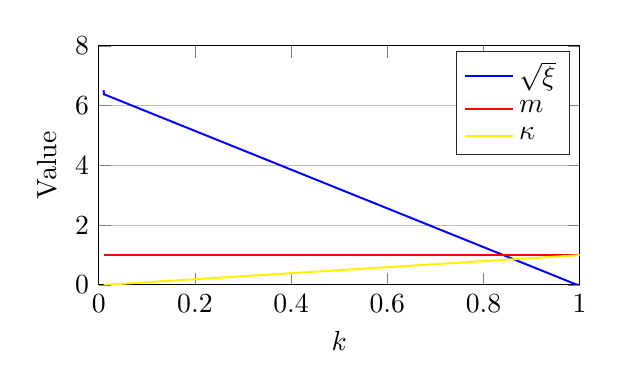
\begin{tikzpicture}

\begin{axis}[%
% width=4.634in,
width=6.634in,
height=3.612in,
at={(2.596in,2.358in)},
% scale only axis,
xmin=0,
xmax=1,
xlabel style={font=\color{white!15!black}},
xlabel={$k$},
xlabel near ticks,
ymin=0,
ymax=8,
ylabel style={font=\color{white!15!black}},
ylabel={Value},
ylabel near ticks,
ymajorgrids,
% scale=0.5,
scale=0.4,
axis background/.style={fill=white},
legend style={legend cell align=left, align=left, draw=white!15!black}
]
\addplot [color=blue, line width = 0.25mm]
  table[row sep=crcr]{%
1	0\\
0.999009009009009	0.00140216778227743\\
0.998018018018018	0.00280572716902405\\
0.997027027027027	0.00421068092522594\\
0.996036036036036	0.00561703182411782\\
0.995045045045045	0.00702478264721581\\
0.994054054054054	0.00843393618435142\\
0.010990990990991	6.37906390177465\\
0.01	6.51269413406059\\
};
\addlegendentry{$\sqrt{\xi}$}

\addplot [color=red, line width = 0.25mm]
  table[row sep=crcr]{%
1	1\\
0.999009009009009	1\\
0.998018018018018	1\\
0.997027027027027	1\\
0.01	1\\
};
\addlegendentry{$m$}

\addplot [color=yellow, line width = 0.25mm]
  table[row sep=crcr]{%
1	1\\
0.999009009009009	0.998019000081162\\
0.998018018018018	0.996039964288613\\
0.997027027027027	0.994062892622352\\
0.010990990990991	0.000120801882964045\\
0.01	0.0001\\
};
\addlegendentry{$\kappa$}

\end{axis}
\end{tikzpicture}%
}}\\
  \vspace{-1cm}
  \subfloat[]{  \resizebox{0.4\textwidth}{!}{% This file was created by matlab2tikz.
%
%The latest updates can be retrieved from
%  http://www.mathworks.com/matlabcentral/fileexchange/22022-matlab2tikz-matlab2tikz
%where you can also make suggestions and rate matlab2tikz.
%
\definecolor{blue}{RGB}{76,100,135}
\definecolor{red}{RGB}{153,0,0}
\definecolor{yellow}{RGB}{227,178,60}
\definecolor{mycolor1}{rgb}{0.00000,0.44700,0.74100}%
\definecolor{mycolor2}{rgb}{0.85000,0.32500,0.09800}%
\definecolor{mycolor3}{rgb}{0.92900,0.69400,0.12500}%
%
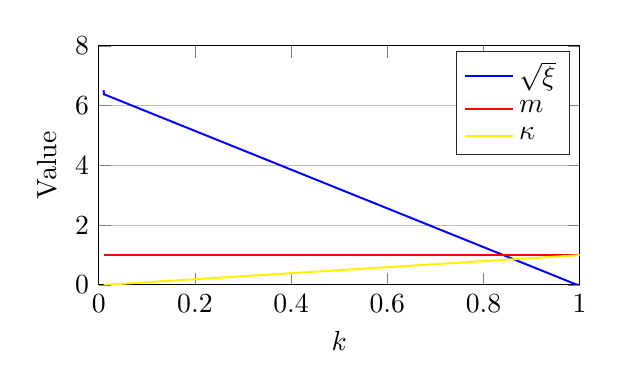
\begin{tikzpicture}

\begin{axis}[%
% width=4.634in,
width=6.634in,
height=3.612in,
at={(2.596in,2.358in)},
% scale only axis,
xmin=0,
xmax=1,
xlabel style={font=\color{white!15!black}},
xlabel={$k$},
xlabel near ticks,
ymin=0,
ymax=8,
ylabel style={font=\color{white!15!black}},
ylabel={Value},
ylabel near ticks,
ymajorgrids,
% scale=0.5,
scale=0.4,
axis background/.style={fill=white},
legend style={legend cell align=left, align=left, draw=white!15!black}
]
\addplot [color=blue, line width = 0.25mm]
  table[row sep=crcr]{%
1	0\\
0.999009009009009	0.00140216778227743\\
0.998018018018018	0.00280572716902405\\
0.997027027027027	0.00421068092522594\\
0.996036036036036	0.00561703182411782\\
0.995045045045045	0.00702478264721581\\
0.994054054054054	0.00843393618435142\\
0.010990990990991	6.37906390177465\\
0.01	6.51269413406059\\
};
\addlegendentry{$\sqrt{\xi}$}

\addplot [color=red, line width = 0.25mm]
  table[row sep=crcr]{%
1	1\\
0.999009009009009	1\\
0.998018018018018	1\\
0.997027027027027	1\\
0.01	1\\
};
\addlegendentry{$m$}

\addplot [color=yellow, line width = 0.25mm]
  table[row sep=crcr]{%
1	1\\
0.999009009009009	0.998019000081162\\
0.998018018018018	0.996039964288613\\
0.997027027027027	0.994062892622352\\
0.010990990990991	0.000120801882964045\\
0.01	0.0001\\
};
\addlegendentry{$\kappa$}

\end{axis}
\end{tikzpicture}%
}}
  \subfloat[]{  \resizebox{0.4\textwidth}{!}{% This file was created by matlab2tikz.
%
%The latest updates can be retrieved from
%  http://www.mathworks.com/matlabcentral/fileexchange/22022-matlab2tikz-matlab2tikz
%where you can also make suggestions and rate matlab2tikz.
%
\definecolor{blue}{RGB}{76,100,135}
\definecolor{red}{RGB}{153,0,0}
\definecolor{yellow}{RGB}{227,178,60}
\definecolor{mycolor1}{rgb}{0.00000,0.44700,0.74100}%
\definecolor{mycolor2}{rgb}{0.85000,0.32500,0.09800}%
\definecolor{mycolor3}{rgb}{0.92900,0.69400,0.12500}%
%
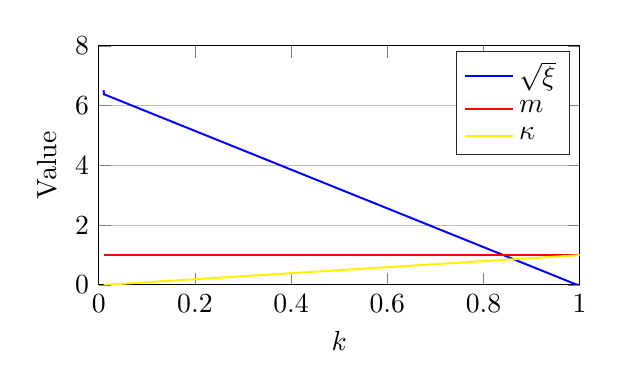
\begin{tikzpicture}

\begin{axis}[%
% width=4.634in,
width=6.634in,
height=3.612in,
at={(2.596in,2.358in)},
% scale only axis,
xmin=0,
xmax=1,
xlabel style={font=\color{white!15!black}},
xlabel={$k$},
xlabel near ticks,
ymin=0,
ymax=8,
ylabel style={font=\color{white!15!black}},
ylabel={Value},
ylabel near ticks,
ymajorgrids,
% scale=0.5,
scale=0.4,
axis background/.style={fill=white},
legend style={legend cell align=left, align=left, draw=white!15!black}
]
\addplot [color=blue, line width = 0.25mm]
  table[row sep=crcr]{%
1	0\\
0.999009009009009	0.00140216778227743\\
0.998018018018018	0.00280572716902405\\
0.997027027027027	0.00421068092522594\\
0.996036036036036	0.00561703182411782\\
0.995045045045045	0.00702478264721581\\
0.994054054054054	0.00843393618435142\\
0.010990990990991	6.37906390177465\\
0.01	6.51269413406059\\
};
\addlegendentry{$\sqrt{\xi}$}

\addplot [color=red, line width = 0.25mm]
  table[row sep=crcr]{%
1	1\\
0.999009009009009	1\\
0.998018018018018	1\\
0.997027027027027	1\\
0.01	1\\
};
\addlegendentry{$m$}

\addplot [color=yellow, line width = 0.25mm]
  table[row sep=crcr]{%
1	1\\
0.999009009009009	0.998019000081162\\
0.998018018018018	0.996039964288613\\
0.997027027027027	0.994062892622352\\
0.010990990990991	0.000120801882964045\\
0.01	0.0001\\
};
\addlegendentry{$\kappa$}

\end{axis}
\end{tikzpicture}%
}}\\
  \vspace{-1cm}
  \subfloat[]{  \resizebox{0.4\textwidth}{!}{% This file was created by matlab2tikz.
%
%The latest updates can be retrieved from
%  http://www.mathworks.com/matlabcentral/fileexchange/22022-matlab2tikz-matlab2tikz
%where you can also make suggestions and rate matlab2tikz.
%
\definecolor{blue}{RGB}{76,100,135}
\definecolor{red}{RGB}{153,0,0}
\definecolor{yellow}{RGB}{227,178,60}
\definecolor{mycolor1}{rgb}{0.00000,0.44700,0.74100}%
\definecolor{mycolor2}{rgb}{0.85000,0.32500,0.09800}%
\definecolor{mycolor3}{rgb}{0.92900,0.69400,0.12500}%
%
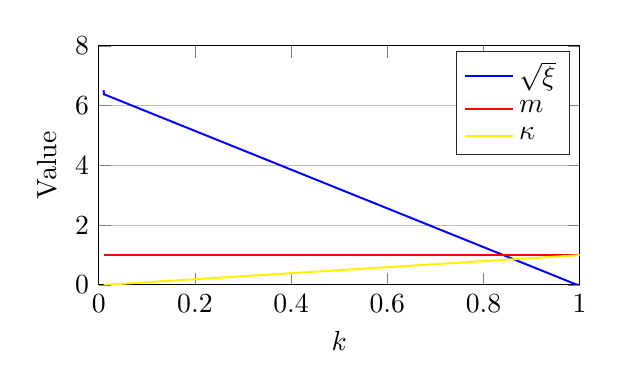
\begin{tikzpicture}

\begin{axis}[%
% width=4.634in,
width=6.634in,
height=3.612in,
at={(2.596in,2.358in)},
% scale only axis,
xmin=0,
xmax=1,
xlabel style={font=\color{white!15!black}},
xlabel={$k$},
xlabel near ticks,
ymin=0,
ymax=8,
ylabel style={font=\color{white!15!black}},
ylabel={Value},
ylabel near ticks,
ymajorgrids,
% scale=0.5,
scale=0.4,
axis background/.style={fill=white},
legend style={legend cell align=left, align=left, draw=white!15!black}
]
\addplot [color=blue, line width = 0.25mm]
  table[row sep=crcr]{%
1	0\\
0.999009009009009	0.00140216778227743\\
0.998018018018018	0.00280572716902405\\
0.997027027027027	0.00421068092522594\\
0.996036036036036	0.00561703182411782\\
0.995045045045045	0.00702478264721581\\
0.994054054054054	0.00843393618435142\\
0.010990990990991	6.37906390177465\\
0.01	6.51269413406059\\
};
\addlegendentry{$\sqrt{\xi}$}

\addplot [color=red, line width = 0.25mm]
  table[row sep=crcr]{%
1	1\\
0.999009009009009	1\\
0.998018018018018	1\\
0.997027027027027	1\\
0.01	1\\
};
\addlegendentry{$m$}

\addplot [color=yellow, line width = 0.25mm]
  table[row sep=crcr]{%
1	1\\
0.999009009009009	0.998019000081162\\
0.998018018018018	0.996039964288613\\
0.997027027027027	0.994062892622352\\
0.010990990990991	0.000120801882964045\\
0.01	0.0001\\
};
\addlegendentry{$\kappa$}

\end{axis}
\end{tikzpicture}%
}}
  \caption{caption text 23}
  \label{fig:compare}
\end{figure}



\chapter{Discussion}
